% Created 2017-03-01 Wed 20:38
\documentclass[10pt]{article}
\usepackage[utf8]{inputenc}
\usepackage[T1]{fontenc}
\usepackage{fixltx2e}
\usepackage{graphicx}
\usepackage{longtable}
\usepackage{float}
\usepackage{wrapfig}
\usepackage{rotating}
\usepackage[normalem]{ulem}
\usepackage{amsmath}
\usepackage{textcomp}
\usepackage{marvosym}
\usepackage{wasysym}
\usepackage{amssymb}
\tolerance=1000
\usepackage{natbib}
\usepackage[linktocpage,pdfstartview=FitH,colorlinks,
linkcolor=blue,anchorcolor=blue,
citecolor=blue,filecolor=blue,menucolor=blue,urlcolor=blue]{hyperref}
\usepackage[margin=2cm]{geometry}
\pagenumbering{gobble}
\usepackage{wrapfig}
\usepackage{multicol}
\setlength\columnsep{20pt}
\author{Alejandro Rodríguez Salamanca - r0650814 - Erasmus}
\date{}
\title{Non-linear regression and classification with MLPs}
\begin{document}

\maketitle

\begin{multicols}{2}

  \section*{Regression}
  In this problem, the objective is to approximate a non-linear function using
  a feedforward artificial neural network. The first step is to build the dataset.
  \subsection*{Define the dataset}
  First, 
  The dataset must be constructed using the digits of the student number. The
  largest five digits in descending order are used, this is, \textbf{86541}, to
  build a target \textit{Tnew}. This target is built using the following formula:

  $$Tnew = (8T_1 + 6T_2 + 5T_3 + 4T_4 + 1T_5) / (8 + 6 + 5 + 4 + 1)$$
  where $T_1, T_2, \ldots, T_5$ are located in the input data file and represents
  5 independent nonlinear functions.

  The dataset to use consists of $X_1, X_2$ and $Tnew$. To draw 3 independent samples
  of 1000 points each, a vector from 1 to 13600 is created. This vector represents
  the indices of the dataset. Then, the content of this vector is randomized, and
  1000 items are selected from $X_1, X_2$ and $Tnew$ using this randomized vector.
  This new dataset is now the training set, validation set, and test set, respectively.

  \section*{Classification}
  Classifitation is a key problem in machine learning. This problem proposes a binary
  classification using a  real-life dataset containing characteristics
  and quality of red and white wine.

  \subsection*{Dataset}
  Given my student number, r065081\textbf{4}, the dataset is constructed in the folliwing way
  using the white whine data:
  \begin{itemize}
    \item For the positive class, $C_{+} = 4$
    \item For the negative class, $C_{-} = 5+6$
    \end{itemize}

    The last column of the data set, indicating the original class, is removed, and
    the new data is labeled using $1$ for the positive class, and $-1$ for the negative
    class.

    The number of instances in each class differs considerably, containing the positive
    class 163 instances and the negative class 3655. 

    \subsection*{Classify}
    First of all, as the classes are unbalanced, it is neccessary to determine whether
    a result is considered good or not. If the majority category is always predicted,
    this is, the prediction is always $C_{-}$ an accuracy in the classification of
    95,73\% is obtained. This result can be considered as our baseline data.
    
    Then, a feedforward neural network is created. Different algorithms and network
    architectures has been tried, and the obtained results are presented:

    \begin{itemize}
    \item \textbf{Number of hidden layers} - Our experiments has shown that with two hidden
      layers, the best results are achieved. Although other architectures with
      one and three hidden layers has been tested, the results did not shown an increase in
      the network performance.
    \item \textbf{Number of neurons in the hidden layers} - The selected number of neurons for the
      first hidden layer is 20, and 8 for the second one. The purpose of this is to
      generalize and find underlying patterns in the data, and use this patterns
      to concretize.
    \item \textbf{Epochs} - The number of epochs has been set to 400.
    \item \textbf{Transfer function} - The transfer function used for the second
      layer is \texttt{tansig}, as the results obtained are slightly better than
      the ones using \texttt{purelin}.
    \end{itemize}

    \begin{center}
    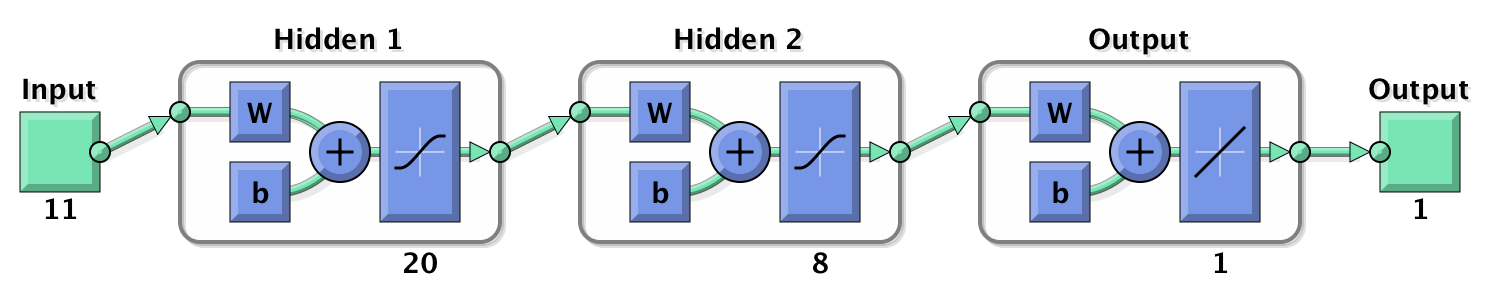
\includegraphics[width=\linewidth]{img/net}
    \end{center}

    Using this network architecture, different training algorithm has been used:

    \begin{itemize}
    \item \texttt{traingd} - Gradient descent is a well-known algorithm that
      has been studied in previous assignments. The main problem of this algorithm
      is that it is prone to got stuck in local minima. In this case, it returns an
      accuracy of 95.73\%, which is the one obtained using ZeroR.
    \item \texttt{trainlm} - Levenberg-Marquardt slightly improves Gradient descent
      with a performance of 95.96\%.
    \item \texttt{trainbr} - Bayesian regularization shows the best results,
      obtaining an accuracy of 98.9\%
    \end{itemize}

    \subsection*{Dimensionality reduction}
    To increase the performance of the network and reduce the complexity
    of the data set, Principal Component Analysis is applied. This method
    reduces the dimensionality of the data. First, we have to see
    which dimensions contains most of the variance, this is, separates the data
    better. It can be done calculating the eigenvalues of the covariance matrix
    of the data, and plotting them.

    % plot eigvals
    \begin{center}
    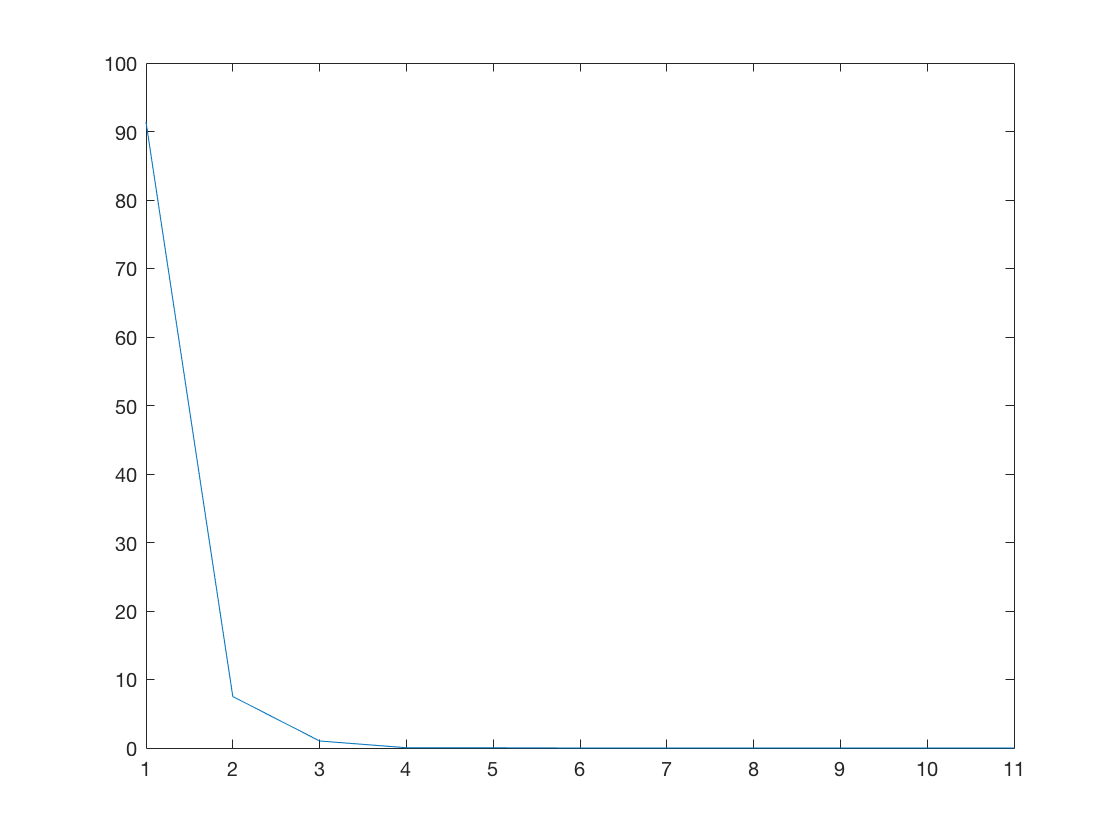
\includegraphics[width=\linewidth]{img/variance}
    \end{center}
    

    It can be seen that the first 4 dimensions holds the majority of the variance,
    which means that the dataset can be reduced from 11 dimensions to 4 without loss
    of generality.

    Now, or dataset has been reduced to 4 dimensions, and a feedforward neural
    network is applied to classificate the new dataset.

    First, the same network with the same parameters and options used before is
    applied, to see the impact of dimensionality reduction in the results.
    Training and executing the network with the reduced dataset returns an
    accuracy of 97.73\%, which is slightly worse than the one obtained with
    the original dataset, but better than the results obtained with ZeroR.

    The network parameters and architecture have been changed, and other approaches
    to improve generalization and avoid overfitting have been tried, such as
    retraining the neural network and using multiple neural networks averaging
    their outputs, but it has not been appreciated an improvement in the accuracy.

  \end{multicols}

  \newpage
  \section*{Appendix}

\end{document}
